\chapter{Methodology}
\label{cha:methods}
In this chapter, we define all the methods and metrics that will be used in the later parts of this thesis. Our goal is to examine a diverse range of techniques to determine what works well and what does not, providing a comprehensive evaluation.

We will explore several prominent classification and regression techniques, including SVM, artificial neural networks, decision trees, and clustering. 

\section{Machine Learning}

In the context of ML, we start with a dataset \( X \) comprising various input-output pairs \((x, y)\). We hypothesize that there exists an underlying function \( f \) which accurately maps any input \( x \) to its corresponding output \( y \). Mathematically, this relationship is expressed as \( f(x) = y \). While the exact form of \( f \) is unknown, we attempt to approximate it with a function \( \hat{f} \). This approximation \( \hat{f} \) is then used to predict outputs \( \hat{y} \) for new inputs \( \hat{x} \).

To assess the performance of our approximation \( \hat{f} \), we employ a loss function \( L(y, \hat{y}) \), which quantifies the discrepancy between the true output \( y \) and the predicted output \( \hat{y} \) ~\cite{murphy2013machine}. The primary objective during the training phase of a machine learning model is to minimize this loss function over the training data, thereby improving the accuracy of our predictions.

The ultimate goal is to ensure that our model makes accurate predictions for new, unseen inputs ~\cite{murphy2013machine}. ML methodologies are broadly classified into two main categories.

\section{Supervised Learning}
The first is called predictive or supervised learning. Here, the goal is to figure out how to map inputs $x$ to outputs $y$, using examples where we already know the answers. We call these examples the training set $D$, and we label it as 
$D = \{(x_i, y_i)\}_{i=1}^N$,
where $N$ is how many data points we have.

In the simplest form, each input 
$x_i$ is a list of numbers, like someone's height and weight. We call these numbers features or attributes. But $x_i$ could be something more complex, like a picture or a sentence. The output 
$y_i$ could be something simple like a category, such as 'male' or 'female', or it could be a number, like for example someone's income level. When $y_i$ is a category, we call the problem classification. When $y_i$ is a number, it's called regression. There is also a special kind called ordinal regression, where the categories have a natural order, like grades from A to F ~\cite{murphy2013machine}.

\section{Classification}

When we have two classes, we usually have \( y \in \{0, 1\} \). This is called binary classification. If we have more than two classes, say \( C \) $\in \mathbb{N}$ classes, then \( y \in \{1, \ldots, C\} \), which is known as multiclass classification ~\cite{murphy2013machine}.

Sometimes, things can belong to more than one class at the same time. For example, someone can be both tall and strong. We call this multi-label classification. Mostly, we focus on predicting one class out of many, which is the multiclass classification ~\cite{murphy2013machine}.

In simple words, classification is about guessing which group, or class, something belongs to, so mathematically
\begin{equation}
    \hat{f}(x) = \underset{y \in Y} \arg \max p(y|x)
\end{equation}
Where $p(y|x)$ represents the probability distribution of the output $y$ given the input $x$ ~\cite{murphy2013machine}.

\subsection{Support Vector Machine}

SVMs are used to classify new given data by finding a hyperplane which separates the training set into different classes.\\ 
In the simple case of a SVM we only have two labels i.e. $Y \in \{0,1 \}^N$ and the space for our training data is given by $[X , Y] \in \mathbb{R}^d \times \{0,1 \}$, where $X$ is our training dataset and $Y$ the target space. The goal of the SVM is now to find a vector $w \in \mathbb{R}^d$ and a offset $b \in\mathbb{R}^d $ s.t. 
\begin{equation}
    \mathrm{sign}(w^T x_i +b) = y_i \qquad i \in \{1, \dots, d\}
\end{equation}
Therefore $w^T x + b = 0$ describes a hyperplane in $\mathbb{R}^d$. \\
In addition we want the hyperplane as far away as possible of both classes of the data.

More precise we want,
\begin{equation}
    (w,b) = \underset{(w,b)}{\mathrm{argmax}} \left (  \min_{(x,y)} \frac{w^T x + b}{ \lVert w \rVert} y \right )
\end{equation}

To optimize this is not easy at all,
therefore we define our minimum distance as $\kappa$. Which means that
\begin{equation}
    \kappa \leq (w^T x + b)y \text{ } \forall x \in X  \iff 1 \leq \left(\frac{w^T x}{\kappa} + \frac{b}{\kappa}\right)y \text{ } \forall x \in X 
\end{equation}
Therefore it is sufficient to optimize $\mathrm{argmax}_w \frac{1}{\lVert w \rVert}$ with the constraint $ 1 \leq (w^T x + b)y$. This can be optimized with help of Lagrange multipliers and gradient descent ~\cite{10.1023/A:1009715923555}. For technical reasons we optimize an equivalent problem, which is given by, 
\begin{equation}
    \underset{(w,b)}{\mathrm{argmin}} \frac{1}{2} \lVert w \rVert^2 \text{ with } 1 \leq (w^T x + b)y \text{ } \forall x \in X 
\end{equation}

Using the Lagrange multipliers method we obtain a linear combination with gives us the best possible hyperplane ~\cite{10.1023/A:1009715923555}. This can be expressed by, 
\begin{equation}
    w^T z + b = \sum_{(x,y)}  y \alpha_x  x^T z +b
\label{eq:SVM}    
\end{equation}
Where $z$ is a new data point and the $\alpha_x$ are the Lagrange multipliers. Note that our hyperplane is only depending on our training data. \\


\FloatBarrier
\begin{figure}[h!]
    \centering
    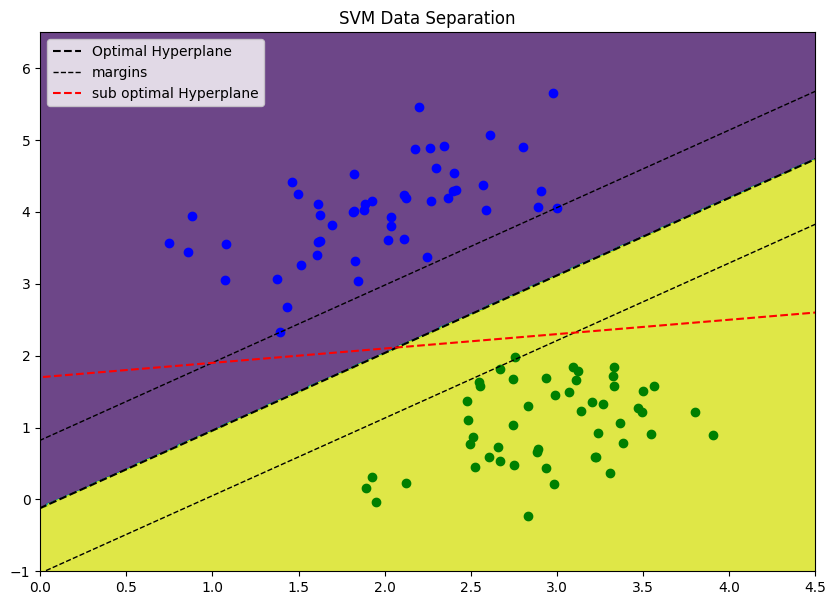
\includegraphics[width=0.7\textwidth]{Master Thesis/Plots/SVM.png}
    \caption{SVM linear dividing the space in to two regions to classify new data. The black line is the best possible line resulting out of a SVM.}
    \label{fig:SVM1}
\end{figure}
\FloatBarrier

Figure ~\ref{fig:SVM1} is an example of how SVM could look like in a visual case.

What is the approach if we have more than two classes? The solution for this problem is to use multiple SVMs, which then in combination can distinguish a single class. 
There are two common approaches: 'one-against-all' and 'one-against-one' ~\cite{PMID:18244442}.
In the one-against-all approach we need $m$ classifier for $m$ classes. The $i$-th classifier separates the $i$-th class from the remaining other $m-1$ classes. \\
The one-against-one approach is to use a classifier to linear separate all pairs of classes. This would need $\frac{m(m-1)}{2}$ classifier and is therefore computational more costly.

\subsection{Ensemble Learning}

In case of a classification task we can train multiple computational efficient, non deterministic models and make a majority vote for the label of a data point. Let $h_1, h_2, \cdots , h_t$ be such classifiers. With $h_{i \in \{1, \dots, t\}}: X \rightarrow Y$, where $X$ is our training dataset and $Y$ is our target space, we can express the majority vote $V(x)$ as 
\begin{equation}
    V(x) = \max_{y \in Y} (h_1(x), h_2(x) , \dots , h_t(x) )
\end{equation}

This diversity of the weak classifiers can lead to astonishing results ~\cite{book}. Examples for weak classifiers are RF and AdaBoost which are both really popular in practice ~\cite{book}.\\
To illustrate why Ensemble Learning can produce excellent results, consider the following example. 
\subsubsection{Wisdom of the Crowd}
Let $Y = \{0,1\}$, let $x_i \in X$ $\subset \mathbb{R}$ be a data point with label $y_i$. Let $\{h_1, \dots , h_t \} = \mathcal{H}$ be the set of classifiers. We assume that,
\begin{equation}
    P(h(x) = y) > \frac{1}{2} \text{ } \forall h \in \mathcal{H}
\label{eq:crowd}    
\end{equation}
Which means that a classifier will be correct more than half of the time.
We then see with Hoeffdings inequality ~\cite{book}, which is given by:
let $X_1, \dots, X_n $ be i.i.d. and there exist $a,b \in \mathbb{R}$ such that $a< X_i <b$, then 
\begin{equation}
    P \left[ \lvert \sum_{i=1}^n (X_i - \mathbb{E}[X_i])\rvert > \epsilon  \right] < 2 \exp \left ( - \frac{2n\epsilon^2}{(b-a)^2} \right )
\label{eq:Hoeffding}    
\end{equation}
that for large enough $t$ the majority vote will be most likely correct. Therefore consider the random variable $h_i$ with 
\begin{equation}
    h_i = 
    \begin{cases}
    1,& \text{if } h_i(x) = y\\
    0,              & \text{otherwise}
\end{cases}
\end{equation}
Since equation \eqref{eq:crowd} holds, we know there exists a $\delta > 0$ with 
$P(h_i) = \frac{1}{2} + \delta = \mathbb{E}[h_i]$. We now want to know what the probability is that the majority vote makes the correct decision i.e. $P\left [\sum_i^t h_i > \frac{t}{2} \right ]$. Taking the opposite event 
\begin{equation*}
    P \left [ \sum_i^t h_i \leq \frac{t}{2} \right] = P \left [ \frac{1}{t} \sum_i^t h_i - \frac{1}{t} \leq 0 \right] \leq P \left [ \lvert \frac{1}{t} \sum_i^t h_i - (\frac{1}{2} + \delta ) \rvert \leq \delta \right]
\end{equation*}

And with Hoeffding it now follows that,
\begin{equation*}
    P \left [ \sum_i^t h_i \leq \frac{t}{2} \right] \leq 2\exp \left ( -2t \delta^2 \right) \xrightarrow{t \rightarrow \inf} 0
\end{equation*}

This shows us, that under the described condition the probability that the majority vote is wrong goes to zero for a large amount of classifiers. However we assumed that our voters are independent, which is usually not the case. It still gives a good justification why Ensemble Learning can be strong. 

\subsection{Random Forest}

Kernel methods can provide a powerful way to create non-linear models for regression and classification. The prediction takes the form:
\begin{equation}
    f(\mathbf{x}) = \mathbf{w}^T \boldsymbol{\phi}(\mathbf{x}),
\end{equation}
where we define
\begin{equation}
    \boldsymbol{\phi}(\mathbf{x}) = [\kappa(\mathbf{x}, \boldsymbol{\mu}_1), \ldots, \kappa(\mathbf{x}, \boldsymbol{\mu}_N)],
\end{equation}
and where $\boldsymbol{\mu}_k$ are either all the training data or some subset.

To estimate the kernel function $\kappa(\mathbf{x}, \mathbf{x}')$, we use the Automatic Relevance Determination kernel:
\begin{equation}
    \kappa(\mathbf{x}, \mathbf{x}') = \theta_0 \exp \left( -\frac{1}{2} \sum_{j=1}^D \theta_j (x_j - x_j')^2 \right).
\end{equation}

An alternative approach is to create an adaptive basis-function model:
\begin{equation}
    f(\mathbf{x}) = w_0 + \sum_{m=1}^M w_m \phi_m(\mathbf{x}),
\end{equation}
where $\phi_m(\mathbf{x})$ is the $m$-th basis function, learned from the data.

Classification and Regression Tree (CART) models, also known as decision trees, recursively partition the input space and define a local model in each resulting region. The model can be written as:
\begin{equation}
    f(\mathbf{x}) = \mathbb{E}[y|\mathbf{x}] = \sum_{m=1}^M w_m \mathbf{I}(\mathbf{x} \in R_m) = \sum_{m=1}^M w_m \phi(\mathbf{x}; \boldsymbol{\nu}_m),
\end{equation}
where $R_m$ is the $m$-th region, $w_m$ is the mean response in this region, and $\boldsymbol{\nu}_m$ encodes the choice of variable to split on and the threshold value.

The process of growing a tree involves finding the optimal partitioning of the data, which is an NP-complete problem. We use a greedy procedure to compute a locally optimal maximum likelihood estimate.

To reduce the variance of an estimate, we average together many estimates. In RF, we train $M$ different trees on different subsets of the data, chosen randomly with replacement, and compute the ensemble:
\begin{equation}
    f(\mathbf{x}) = \frac{1}{M} \sum_{m=1}^M f_m(\mathbf{x}),
\end{equation}
where $f_m$ is the $m$-th tree. This technique is known as \textit{bagging} (bootstrap aggregating).

The split function chooses the best feature $j^*$ and the best value for that feature $t^*$:
\begin{equation}
    (j^*, t^*) = \arg \min_{j \in \{1, \ldots, D\}, t \in \mathcal{T}_j} \left[ \min \text{cost} \left( \{x_i, y_i : x_{ij} \leq t \} \right) + \text{cost} \left( \{x_i, y_i : x_{ij} > t \} \right) \right],
\end{equation}
where $\mathcal{T}_j$ is the set of possible thresholds for feature $j$.

In the regression setting, we define the cost as:
\begin{equation}
    \text{cost}(\mathcal{D}) = \sum_{i \in \mathcal{D}} (y_i - \bar{y})^2,
\end{equation}
where $\bar{y}$ is the mean of the response variable in the specified set of data.

In the classification setting, we measure the quality of a split using:
\begin{equation}
    \hat{\pi}_c = \frac{1}{|\mathcal{D}|} \sum_{i \in \mathcal{D}} \mathbf{I}(y_i = c),
\end{equation}
and evaluate the partition using the Gini index:
\begin{equation}
    G = \sum_{c=1}^C \hat{\pi}_c (1 - \hat{\pi}_c).
\end{equation}

Despite its effectiveness, RF may produce highly correlated predictors if the same algorithm is run on similar data subsets. To mitigate this, the technique uses a random subset of variables for each tree construction, known as \emph{random forests}, which enhances the model's predictive power across various applications ~\cite{murphy2013machine}.

\FloatBarrier
\begin{figure}[h!]
    \centering
    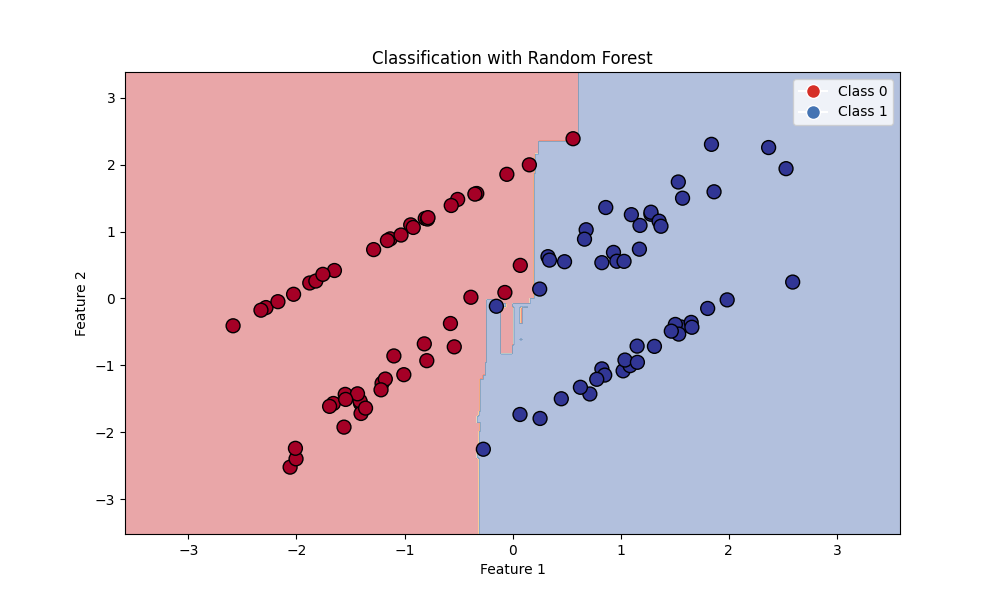
\includegraphics[width=0.8\textwidth]{Master Thesis/Plots/randomForestexample.png}
    \caption{RF separating data points into two classes}
    \label{fig:RF}
\end{figure}
\FloatBarrier

Figure ~\ref{fig:RF} is an example of how classification with RF could look like in a visual case.

\subsection{Boosting as Functional Gradient Descent}

\subsubsection*{Gradient Descent}
Gradient descent is a fundamental algorithm for unconstrained optimization. It iterative updates parameters to minimize a given function \( f(\theta) \). The update rule for gradient descent is given by:
\begin{equation}
    \theta_{k+1} = \theta_k - \eta_k g_k,
\end{equation}
where \( \eta_k \) is the step size or learning rate, and \( g_k \) is the gradient of \( f \) at \( \theta_k \).

Choosing an appropriate step size \( \eta_k \) is crucial because if \( \eta_k \) is too small, the convergence will be very slow.
But if \( \eta_k \) is too large, the algorithm may oscillate or diverge ~\cite{murphy2013machine}.

\subsubsection*{Gradient Boosting}
A more generalized approach, known as gradient boosting, was developed to extend boosting capabilities across various loss functions. It conceptualizes the problem as a functional gradient descent. This builds on the principles of ensemble learning, which have been discussed previously. Ensemble learning involves combining multiple models to improve performance, while boosting is a method that sequentially adjusts the weights of weak learners to minimize errors. It conceptualizes the problem as a functional gradient descent:
\begin{equation}
\hat{f} = \arg\min_{f} L(f)
\end{equation}
Here, $f = (f(x_1), \dots, f(x_d))$ represents the parameters, $f$ is a possible outcome of the ensemble learning method and $L$ represents the loss function. The method updates predictions in a stage wise manner by moving in the direction that reduces the loss function, effectively performing gradient descent in function space. Each update is formulated as:

\begin{equation}
f_m = f_{m-1} - \rho_m g_m
\end{equation}
where $\rho_m$ is the learning rate and $g_m$ is the gradient, optimized as:
\begin{equation}
\rho_m = \arg\min_{\rho \in \mathbb{R}} L(f_{m-1} - \rho g_m)
\end{equation}
The weak learner fits each update to approximate the negative gradient of the loss function, enhancing the model's ability to generalize beyond the fixed set of training points ~\cite{murphy2013machine}.

\subsection{XGBoost}

Extreme Gradient Boosting (XGBoost) is renowned for its efficiency, scalability, and robust handling of sparse data and missing values. It incorporates regularization to prevent overfitting and uses parallel and distributed computing to speed up training. XGBoost's unique features include the 'weighted quantile sketch' for handling weighted data, backward pruning to remove unnecessary splits, and support for custom loss functions. Its built-in cross-validation and feature importance scores aid in model evaluation and interpretation, making it highly effective for large-scale and complex ML tasks.

The ensemble's power is further harnessed through gradient boosting, a technique that evolves in three steps:

\begin{enumerate}
    \item An initial model $F_0$ is formulated to predict the target variable $y$, generating residuals $(y - F_0)$.
    \item A new model $h_1$ is fitted to these residuals.
    \item The model $F_0$ is then updated with $h_1$ to yield a superior model $F_1$, which exhibits a lower mean squared error compared to $F_0$:
\end{enumerate}

\[
F_1(x) \leftarrow F_0(x) + h_1(x)
\]

The process continues by modeling after the residuals of $F_1$ to construct a new model $F_2$, and this iterative process is carried out for 'm' iterations:

\[
F_2(x) \leftarrow F_1(x) + h_2(x)
\]

\[
\vdots
\]

\[
F_m(x) \leftarrow F_{m-1}(x) + h_m(x)
\]

Throughout this iterative process, the additive learners contribute unique information, enhancing the model's accuracy without altering the functions established in the previous steps ~\cite{analyticsvidhyaIntroductionXGBoost}.
The XGBoost can be used for classification and regression. Figure ~\ref{fig:XGBoost} demonstrates the XGBoost for a classification problem:

\FloatBarrier
\begin{figure}[h!]
  \centering
    \centering
    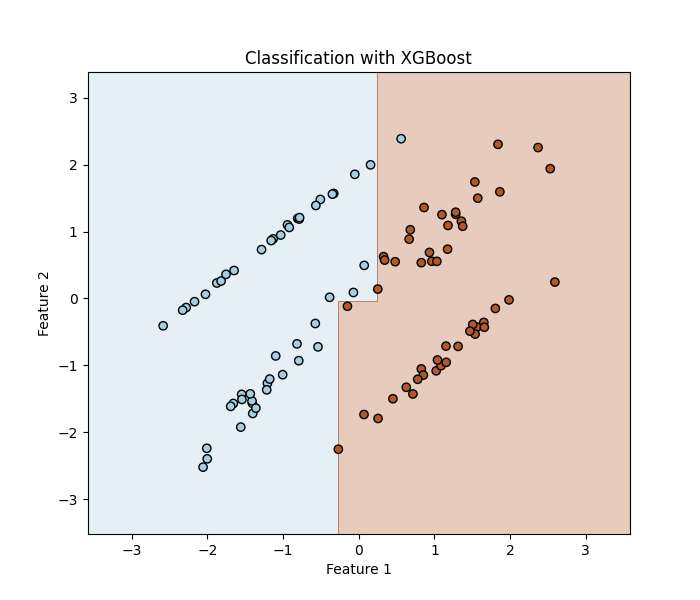
\includegraphics[width=.9\linewidth]{Master Thesis/Plots/classification_with_xgboost.png}
    \caption{XGBoost separating data points into two classes}
    \label{fig:XGBoost}
\end{figure}
\FloatBarrier
We clearly see in figure ~\ref{fig:XGBoost} that XGBoost creates complex decision boundaries for the classification.
This visualization may help later in this work.

\subsection{CatBoost: Gradient Boosting with Decision Trees}
CatBoost is a sophisticated implementation of gradient boosting that utilizes binary decision trees as base predictors. It follows the principles of gradient boosting but introduces several improvements and optimizations for better handling categorical features and preventing overfitting.

The process begins with an initial model \( F_0 \) and iteratively enhances it by fitting subsequent models \( h_t \) to the residuals. CatBoost optimizes this process by employing oblivious decision trees, which apply the same splitting criterion across an entire level of the tree. This leads to more balanced structures and efficient computations.

A decision tree in CatBoost can be defined as:
\begin{equation}
h(x) = \sum_{j=1}^J b_j \mathbbm{1}\{x \in R_j\}
\end{equation}
where \( R_j \) are the disjoint regions of the feature space corresponding to the leaves, and \( b_j \) represents the output value for each region ~\cite{prokhorenkova2019catboost}.

\section{Regression}

\subsection{Logistic Regression}

Logistic regression is a generalization of linear regression for binary classification. Instead of using a Gaussian distribution for the response variable \( y \), we use a Bernoulli distribution since \( y \in \{0, 1\} \). This can be expressed as:
\begin{equation}
    p(y|\mathbf{x}, \mathbf{w}) = \text{Ber}(y|\mu(\mathbf{x})),
\end{equation}
where
\begin{equation}
    \mu(\mathbf{x}) = \mathbb{E}[y|\mathbf{x}] = p(y = 1|\mathbf{x}).
\end{equation}

We compute a linear combination of the inputs, and pass this through the sigmoid function to ensure \( 0 \leq \mu(\mathbf{x}) \leq 1 \):
\begin{equation}
    \mu(\mathbf{x}) = \sigma(\mathbf{w}^T \mathbf{x}),
\end{equation}
where the sigmoid function, also known as the logistic or logit function, is defined as:
\begin{equation}
    \sigma(\eta) = \frac{1}{1 + \exp(-\eta)} = \frac{e^\eta}{e^\eta + 1}.
\end{equation}

Putting these steps together, we get:
\begin{equation}
    p(y|\mathbf{x}, \mathbf{w}) = \text{Ber}(y|\sigma(\mathbf{w}^T \mathbf{x})).
\end{equation}

This is called \textit{logistic regression} due to its similarity to linear regression, although it is a form of classification, not regression.

An example of logistic regression is given by:
\begin{equation}
    p(y_i = 1|x_i, \mathbf{w}) = \sigma(w_0 + w_1 x_i),
\end{equation}
where \( x_i \) is the SAT score of student \( i \) and \( y_i \) indicates whether they passed or failed a class.

The decision rule is defined as:
\begin{equation}
    \hat{y}(\mathbf{x}) = 1 \iff p(y = 1|\mathbf{x}) > 0.5.
\end{equation}

The decision boundary is given by:
\begin{equation}
    \sigma(w_0 + w_1 x) = 0.5 \implies x = x^*.
\end{equation}

Overfitting occurs when a model fits the training data too well, capturing noise instead of the underlying pattern. This can be mitigated by using techniques such as cross-validation and regularization.

Model selection involves choosing the best model from a set of candidates by evaluating their performance on a validation set. This process aims to balance model complexity and accuracy to prevent both overfitting and underfitting ~\cite{murphy2013machine}.

\subsection{Linear Regression}

Regression analysis is very similar to classification. The main difference however is, it is dealing with a continuous response variable ~\cite{murphy2013machine}. Imagine in general having a single real-valued input $x_i \in \mathbb{R}^d$, and a corresponding real-valued response $y_i \in \mathbb{R}$. We explore fitting two models to this data: a linear model (a straight line) and a non-linear model (a quadratic function). The methodologies for fitting these models are discussed subsequently. This simple example can be extended in various ways to include challenges such as high-dimensional inputs, outliers, or non-smooth responses.

Linear regression is one of the most commonly used models in statistical modeling and ML. It posits that the dependent variable, often referred to as the response, is a linear combination of the input variables. The mathematical representation of a linear regression model can be expressed as follows:

\begin{equation}
    f(\mathbf{x}) = \mathbf{w}^T \mathbf{x} + \mathbf{\epsilon} \qquad, \mathbf{w} \in \mathbb{R}^{d} \qquad , \mathbf{x} \in \mathbb{R}^d
\end{equation}

Here, $f(\mathbf{x})$ represents the predicted response for the input vector $\mathbf{x}$, $\mathbf{w}^T \mathbf{x}$ denotes the inner or scalar product of the input vector $\mathbf{x}$ with the model's weight vector $\mathbf{w}$, and $\mathbf{\epsilon}$ symbolizes the residual error, which accounts for the discrepancy between our linear predictions and the actual response. This formula describes the multidimensional case. The equation can be expanded as:

\begin{equation}
    f(\mathbf{x}) = \sum_{j=1}^d w_j x_j + \epsilon_{j}
\end{equation}

where $d$ is the number of features, $w_j$ are the coefficients that represent the weights assigned to each input feature $x_j$, and $\epsilon$ is the error term that captures any factors not explained by the linear model ~\cite{murphy2013machine}.

\FloatBarrier
\begin{figure}[h!]
    \centering
    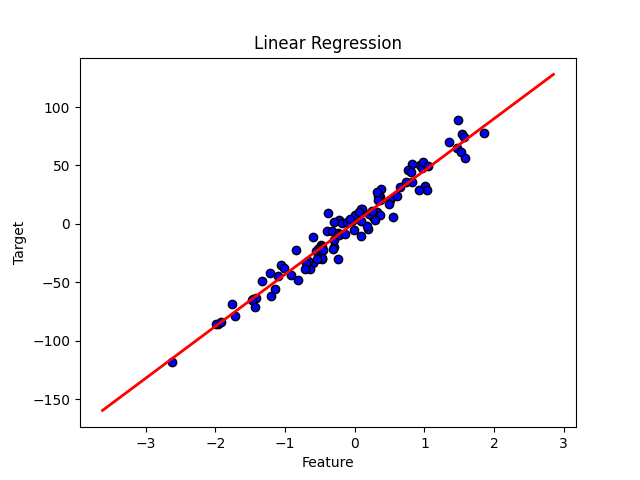
\includegraphics[width=0.7\textwidth]{Master Thesis/Plots/linearregressionexample.png}
    \caption{Linear regression method finding a line trough the data points}
    \label{fig:linreg}
\end{figure}
\FloatBarrier

Figure ~\ref{fig:linreg} is an example of how linear regression could look like in a visual case.

A optimization of this is an approach called boosting. The essence of boosting is to fit adaptive basis-function models, where the functions $\phi_m$ are generated by an algorithm known as a weak learner or a base learner. The algorithm repeatedly applies the weak learner to weighted versions of the data. Initially, all data points are given equal weights, but as the iterations proceed, higher weights are assigned to examples that were incorrectly classified, thus focusing the learning more on harder cases ~\cite{murphy2013machine}.

\section{Artificial Neural Networks}

Artificial Neural Networks (ANNs) are computational models inspired by the human brain, designed to learn complex patterns from data. These networks are composed of layers of interconnected units called neurons, each connection associated with a weight. A prominent type of ANN is the Multilayer Perceptron (MLP), which consists of an input layer, one or more hidden layers, and an output layer. Each layer has neurons connected by weighted links, and the goal is to learn these weights to make accurate predictions.

The MLP can be mathematically represented as follows: For an MLP with \( n \) hidden layers, the function \( F_\theta(x) \) is given by \( F_\theta(x) = f_{n+1}(w_{n+1} f_n(w_n f_{n-1}(\cdots f_1(w_1 x + b_1) + b_2) \cdots + b_{n}) + b_{n+1}) \). Here, \( x \) is the input vector, \( w_i \) are the weight matrices, \( b_i \) are the bias vectors, and \( f_i \) are the activation functions for each layer.

Training an MLP involves adjusting these weights and biases to minimize the error between predicted and actual outputs, using an optimization algorithm like gradient descent. The weight update rule in gradient descent is \( w_{ij}^{(t+1)} = w_{ij}^{(t)} - \eta \frac{\partial L}{\partial w_{ij}} \), where \( \eta \) is the learning rate and \( L \) is the loss function.

Activation functions introduce non-linearity into the model, allowing it to learn complex patterns. Common activation functions include the sigmoid function \( \sigma(x) = \frac{1}{1 + e^{-x}} \) and the ReLU function \( \text{ReLU}(x) = \max(0, x) \) ~\cite{NNs}.

\section{Unsupervised Learning}

Unsupervised learning involves analyzing data without labeled responses, aiming to discover 'interesting structures' within the data, a process often referred to as knowledge discovery. Unlike supervised learning, which requires input-output pairs for training, unsupervised learning focuses on modeling the probability distribution $p(x_i|\phi)$ of the data, without specific targets. Where \(\phi\) represents the parameters of the model that describe the distribution \( p(x_i|\phi) \). These are the unknown parameters that the model adjusts during training to approximate the probability distribution of the data \( x_i \).
This approach is more typical of human and animal learning and is widely applicable, as it doesn't need a human expert to provide labeled data ~\cite{murphy2013machine}.

\subsection{Clustering}

The k-means algorithm works on a set $X$ $\subset$ $\mathbb{R}^d$, which represents an embedding of the vertices. The goal is to find a set of $k$ cluster centers $\mu_C_1$$, \dots ,$$ \mu_C_n$ $\subset$ $\mathbb{R}^d$. The corresponding clusters are then given by 
\begin{equation}
    C_i = {\{x \in X : \lVert x - \mu_{C_i} \rVert}_2 < {\lVert x - \mu_{C_j} \rVert}_2 j \neq i , j\in \{1,\dots ,k\}\}
\end{equation}

If a point is on the boundary between two clusters, it is randomly assigned to one of the adjacent clusters.
We start with a random set of cluster centers and calculate their corresponding clusters.
After that, we calculate new cluster centers from the obtained clusters like 
\begin{equation}
    \mu_{C_i} = \Big(\,\frac{1}{|C_i|}\Big)\,\sum_{x \in C_i}x
\end{equation} 
where $i \in \{1, \dots, k\}$.
We repeat this process until the clusters do not change.
For the k-means algorithm we have a set $X$ consisting of data points and a set $\mu_C$ $\subset$ $V$ representing the centers ~\cite{murphy2013machine}. 

\FloatBarrier
\begin{figure}[h!]
    \centering
    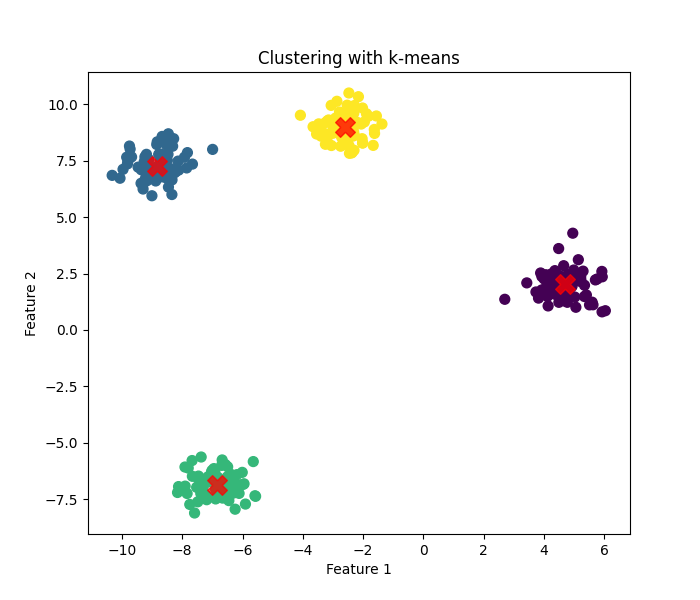
\includegraphics[width=0.7\textwidth]{Master Thesis/Plots/Clustering_Example.png}
    \caption{Method k-means clustering the data points into four clusters}
    \label{fig:clustering}
\end{figure}
\FloatBarrier

Figure ~\ref{fig:clustering} shows the results of a k-means clustering model that groups data points into four clusters. The differences to the previous plots of the methods are that this plot does not show decision boundaries, but the grouping of the data points into clusters.

\subsection{Hierarchical Clustering}

Hierarchical clustering is a method of cluster analysis which seeks to build a hierarchy of clusters. This approach can be categorized into two main types: agglomerative (bottom-up) and divisive (top-down).

Agglomerative clustering, or bottom-up clustering, starts with each object in a singleton cluster. The clusters are iteratively merged based on their similarity until a single cluster containing all objects is formed. 

Initially, each data point \( x_i \) is treated as a singleton cluster \( C_i = \{i\} \). At each step, the two most similar clusters \( C_j \) and \( C_k \) are identified and merged to form a new cluster \( C_\ell = C_j \cup C_k \). The similarity \( d_{jk} \) between clusters is determined using a dissimilarity matrix. After merging \( C_j \) and \( C_k \) into \( C_\ell \), the dissimilarity matrix is updated to reflect the distances between the new cluster \( C_\ell \) and the remaining clusters. Different linkage criteria can be used to define the distance between clusters: 

\textit{Single Linkage}: 
\[ d(C_\ell, C_i) = \min \{d(x_p, x_q) | x_p \in C_\ell, x_q \in C_i\} \]

\textit{Complete Linkage}: 
\[ d(C_\ell, C_i) = \max \{d(x_p, x_q) | x_p \in C_\ell, x_q \in C_i\} \]

\textit{Average Linkage}: 
\[ d(C_\ell, C_i) = \frac{1}{|C_\ell||C_i|} \sum_{x_p \in C_\ell} \sum_{x_q \in C_i} d(x_p, x_q) \]

where $x_p$ and $x_q$ are data points in clusters $C_\ell$ and $C_i$ respectively. This criterion measures the minimum distance between any pair of points in the two clusters.
 
The process is repeated until all points are merged into a single cluster or the desired number of clusters is achieved.

The algorithm for divisive clustering can be summarized as follows:

\FloatBarrier
\begin{algorithm}
\caption{Agglomerative clustering}
\begin{algorithmic}[1]
\State initialize clusters as singletons: for \(i \leftarrow 1\) to \(n\) do \(C_i \leftarrow \{i\}\);
\State initialize set of clusters available for merging: \(S \leftarrow \{1, \ldots, n\}\);
\Repeat
\State Pick 2 most similar clusters to merge: \((j, k) \leftarrow \arg \min_{j,k \in S} d_{jk}\);
\State Create new cluster \(C_\ell \leftarrow C_j \cup C_k\);
\State Mark \(j\) and \(k\) as unavailable: \(S \leftarrow S \setminus \{j, k\}\);
\If {$C_\ell \neq \{1, \ldots, n\}$} 
\State Mark \(\ell\) as available, \(S \leftarrow S \cup \{\ell\}\);
\ForAll {$i \in S$}
\State Update dissimilarity matrix \(d(i, \ell)\);
\EndFor
\EndIf
\Until {no more clusters are available for merging};
\end{algorithmic}
\end{algorithm}
\FloatBarrier

Divisive clustering, or top-down clustering, works in the opposite manner. It starts with all data points in a single cluster and recursively splits them into smaller clusters. This approach is less commonly used due to its computational complexity ~\cite{murphy2013machine}.

Hierarchical clustering provides a comprehensive way to understand the structure within data by creating nested clusters. The choice between agglomerative and divisive methods, as well as the linkage criteria, can significantly impact the resulting hierarchy and its interpretation ~\cite{murphy2013machine}.

\section{Metrics}

To evaluate the performance of classification models in data science and ML, the three metrics precision (p), recall (r) and the f1-score are particularly useful. 
In general when we need to define that TP stands for true positive, FP for false positive and FN for false negative. 

Precision tells us how many of the cases classified as positive are actually positive. For example, we have a group of healthy and sick people and use a program that classifies as either 'healthy' or 'sick'. Precision is then calculated as follows: Of all the people classified as 'sick', how many are actually sick? Described as a mathematical formula it would look like this ~\cite{10.1007/978-3-540-31865-1_25}: 

\begin{equation}
    p = \frac{TP}{TP + FP}
\end{equation}

Recall measures how well the model has captured all actual positive cases. In the example with the healthy and sick people program, this would be: Of all really sick people, how many did the program correctly identify as 'sick'? Mathematically this would be ~\cite{10.1007/978-3-540-31865-1_25}: 

\begin{equation}
    r = \frac{TP}{TP + FN}  
\end{equation}

If you want to measure the balance between precision and recall in a single metric, one can use the f-score. It is particularly useful if a balanced relationship between precision and recall is to be achieved. The f-score is, so to speak, the weighted harmonic average of precision and recall. A higher f-score indicates a better overall performance of the model.
~\cite{10.1007/978-3-540-31865-1_25}:

\begin{equation}
    f_\beta = (1 + \beta^2) \frac{p \cdot r}{(r + \beta^2 p)} \qquad , \beta \in [0 , 1]
\end{equation}

Where $\beta = 1$ represents the f1 score.

The silhouette score is a measure of how similar an object is to its own cluster compared to other clusters. The silhouette scores ranges from $[-1 ,1]$, where a higher value indicates that the object is well matched to its own cluster. The silhouette score of a data point $x$ is given as ~\cite{SilhotteCoefficient}:
\begin{equation}
     s(i) = \frac{b(x) - a(x)}{max\{a(x),b(x)\}}
\end{equation}
with $b(x)$ denoting the mean distance to all other points of the next nearest cluster, and $a(x)$ is the mean distance to all other points of the same cluster. 
The silhouette score for a set of samples is then defined as :
\begin{equation}
    s_C = \frac{1}{n_C} \sum_{x \in C} s(x)
\end{equation}
the mean of the silhouette score for each sample.

Before we introduce \( R^2 \) in this work, we need to mention residuals. 
Residuals are the differences between the observed values \( y_i \) and the predicted values \( \hat{y}_i \) produced by the regression model. Mathematically, the residual for each observation \( i \) is given by ~\cite{Weisberg}:

\[
\text{residual}_i = y_i - \hat{y}_i
\]

The residual sum of squares (\( \text{SS}_{\text{res}} \)) is then calculated by summing the squares of these residuals for all observations:

\[
\text{SS}_{\text{res}} = \sum_{i=1}^{n} (y_i - \hat{y}_i)^2
\]

This measure indicates the extent to which the predicted values differ from the actual observed values. A smaller \( \text{SS}_{\text{res}} \) implies that the model's predictions are closer to the actual data points, indicating a better fit.

The term \(\text{SS}_{\text{tot}}\) refers to the total sum of squares, which measures the total variance in the observed data. It is calculated by summing the squares of the differences between each observed value and the mean of the observed values \(\bar{y}\):

\[
\text{SS}_{\text{tot}} = \sum_{i=1}^{n} (y_i - \bar{y})^2
\]

This term represents the total variation present in the data, without considering the regression model.

Now the coefficient of determination \( R^2 \) can be introduced. It quantifies the proportion of the variance in the dependent variable that is predictable from the independent variables. It is given by ~\cite{Weisberg}:

\[
R^2 = 1 - \frac{\text{SS}_{\text{res}}}{\text{SS}_{\text{tot}}}
\]

An \( R^2 \) value of 1 indicates that the regression model perfectly explains the variance in the data, while an \( R^2 \) value of 0 indicates that the model does not explain any of the variance in the data.

We also used MSE in this work to find out the fact how far apart the real value and the predicted value are. It is calculated like this:
\[
\text{MSE} = \frac{1}{n} \sum_{i=1}^{n} (y_i - \hat{y}_i)^2
\]
This measures the average of the squares of the errors (residuals), which are the differences between the observed values \(y_i\) and the predicted values \(\hat{y}_i\).

Some other measurement is the root-mean-square error (RMSE). It provides a measure of the average magnitude of the prediction error. It is calculated as the square root of the average squared differences between the predicted and actual values:

\[
\text{RMSE} = \sqrt{\frac{\sum_{i=1}^n (y_i - \hat{y}_i)^2}{n}}
\]

\subsection{Cross Entropy}

To measure the differences between two discret probability distributions, p and q, the Kullback-Leibler divergence or relative entropy is often used. 
Mathematically it can be described like this ~\cite{murphy2013machine}: 
\begin{equation}
    \mathbb{KL}(p||q) \equiv \sum_{k=1}^{K} p_k \log \frac{p_k}{q_k}
\end{equation}
where the sum is given by an integral for probability distribution functions. It can be rewritten as:
\begin{equation}
   \mathbb{KL}(p||q) = \sum_k p_k \log p_k - \sum_k p_k \log q_k = -\mathbb{H}(p) + \mathbb{H}(p, q)
\end{equation}
Where $\mathbb{H}(p, q)$ is called the cross entropy (CE).

\begin{equation}
    \mathbb{H}(p, q) \equiv -\sum_k p_k \log q_k
\end{equation}

The CE method is mainly used for combinatorial and multi-extreme optimization as well as for the simulation of rare events. 
With the CE method, a random data sample is generated in each iteration. The parameters of the random mechanism are then updated on the basis of this data in order to generate a 'better' sample in the next iteration. The method uses the Kullback-Leibler distance to minimize the distance between the current estimate and the optimal solution.
This guarantees a more precise estimate of the probabilities searched for ~\cite{crossentropy1}.

\subsection{Silhouette Score and Davies-Bouldin Score}

The silhouette score is a measure of how similar an object is to its own cluster compared to other clusters. The silhouette scores ranges from $[-1 ,1]$, where a higher value indicates that the object is well matched to its own cluster. The silhouette score of a data point x is given as:
\begin{equation}
     s(i) = \frac{b(x) - a(x)}{max\{a(x),b(x)\}}
\end{equation}
with $b(x)$ denoting the mean distance to all other points of the next nearest cluster, and $a(x)$ is the mean distance to all other points of the same cluster. 
The silhouette score for a set of samples is then defined as :
\begin{equation}
    s_C = \frac{1}{n_C} \sum_{x \in C} s(x)
\end{equation}
the mean of the silhouette score for each sample ~\cite{SilhotteCoefficient}.

The Davies-Bouldin score is a measure used to evaluate the quality of clustering by assessing the similarity between clusters. It quantifies how well-separated and compact the clusters are within a dataset. The Davies-Bouldin score is defined based on the following components:

Firstly, the dispersion measure (\( S_i \)) for a cluster \( C_i \) is calculated to determine the spread of data points within the cluster. This is given by:
\[ 
S_i = \left( \frac{1}{|C_i|} \sum_{x \in C_i} \| x - A_i \|^2 \right)^{1/2} 
\]
where \( A_i \) is the centroid of cluster \( C_i \).

Secondly, the separation measure (\( M_{ij} \)) between clusters \( C_i \) and \( C_j \) is determined by the distance between their centroids:
\[ 
M_{ij} = \| A_i - A_j \| 
\]

Using these measures, the similarity measure (\( R_{ij} \)) between clusters \( C_i \) and \( C_j \) is defined as:
\[ 
R_{ij} = \frac{S_i + S_j}{M_{ij}} 
\]

The Davies-Bouldin score for a set of clusters is then calculated as the average similarity of each cluster with its most similar cluster:
\[ 
DBI = \frac{1}{d} \sum_{i=1}^{d} \max_{j \neq i} R_{ij} 
\]
where \( d \) is the total number of clusters.

A lower DBI indicates better clustering performance, with well-separated and compact clusters, while a higher DBI suggests poorer clustering with less distinct clusters. The DBI is effective for comparing the quality of different clustering algorithms or parameter settings and is applicable to datasets of arbitrary dimensionality. This measure requires minimal user interaction and is computationally feasible for large datasets, making it a valuable tool for automated clustering evaluation
~\cite{4766909}.

We have now defined and explained all the methods and metrics that are relevant to the following sections of this paper. By establishing a clear understanding of these techniques, we are now in a position to proceed with the analysis and evaluation of our data. Based on this, we can fully evaluate the effectiveness of different ML approaches in health monitoring and prediction.